\section{Tracking System}

\subsection{Introduction}

To be able to accurately produce a virtual volumetric screen, we need to be able to track the user's face and hands. This is so we can render the correct perspective of the screen to the user. Our tracking system had to fit the following requirements:
\begin{itemize}[itemsep=-0.25em]
	\item \textbf{High resolution:} To be able to accurately track the user's face and hands smoothly.
	\item \textbf{High framerate:} To be able to track the user's face and hands smoothly.
	\item \textbf{Low latency:} To be able to track the user's face and hands in near real-time.
\end{itemize}
%%%%%%%%%%%%%%%%%%%%%%%%%%%%%%%%%%%%%%%%%%%%%%%%%%%%%%%%%%%%%%%%%%%%%%%%%%%%%%%%%%%%%%%%%%%%

\subsection{Hardware}

\begin{figureBox}[label={fig:kinect}, width=0.5\linewidth]{Azure Kinect}
    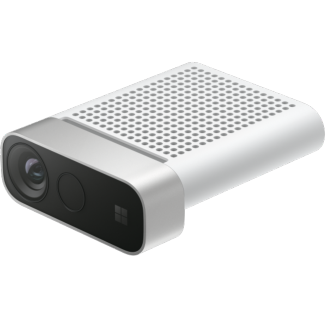
\includegraphics[width = 0.8\linewidth]{./implementation/figures/kinect.pdf}
\end{figureBox}
\textcolor{red}{Get Image from here https://deviestore.com/product/microsoft-azure-kinect/ source microsoft for the image.} \\

For this project we used a Microsoft Azure Kinect camera \tocite Fig~\ref{fig:kinect}. The Azure Kinect camera has two sensors, a depth sensor (IR Sensor) and a colour sensor. For this project we have configured the camera to capture images at its widest field of view $90^{\circ} \times 74.3^{\circ} $, with the exposure time 12.8 ms and it's highest framerate 30fps. To be able to use these settings we had to compromise on the resolution of the images running the RGB camera at $2048 \times 1536$ rather than it's maximum resolution of $4096 \times 3072$ and the depth camera at $2\times2$ binned with a resolution of $512 \times 512$ rather than it's maximum unbinned resolution of $1024 \times 1024$. Because we use the depth camera in wide field of view mode $120^{\circ} \times 120^{\circ} $ rather than $75^{\circ} \times 65^{\circ} $ we compromised on the maximum operating range of the camera only being able to track hands up to 2.88m away rather than 5.46m. \\


%%%%%%%%%%%%%%%%%%%%%%%%%%%%%%%%%%%%%%%%%%%%%%%%%%%%%%%%%%%%%%%%%%%%%%%%%%%%%%%%%%%%%%%%%%%%

\subsection{Core Libaries}  
\begin{figureBox}[label={fig:core-libs}, width=0.8\linewidth]{Core Libraries used for tracking}
    
\includegraphics[width = 1.0\linewidth]{./implementation/figures/libs.png}
\end{figureBox}

\textcolor{red}{Cite libraries for the images}

\subsubsection{Azure Kinect SDK (K4A)}

We use the Azure Kinect SDK (K4A) library to retrieve Captures from the Kinect and the handle the "space" transformations you need to calculate the positions of points in 3D.

\begin{figureBox}[label={fig:diff-spaces}, width=0.8\linewidth]{Different spaces changing Depth and Colour Images}
    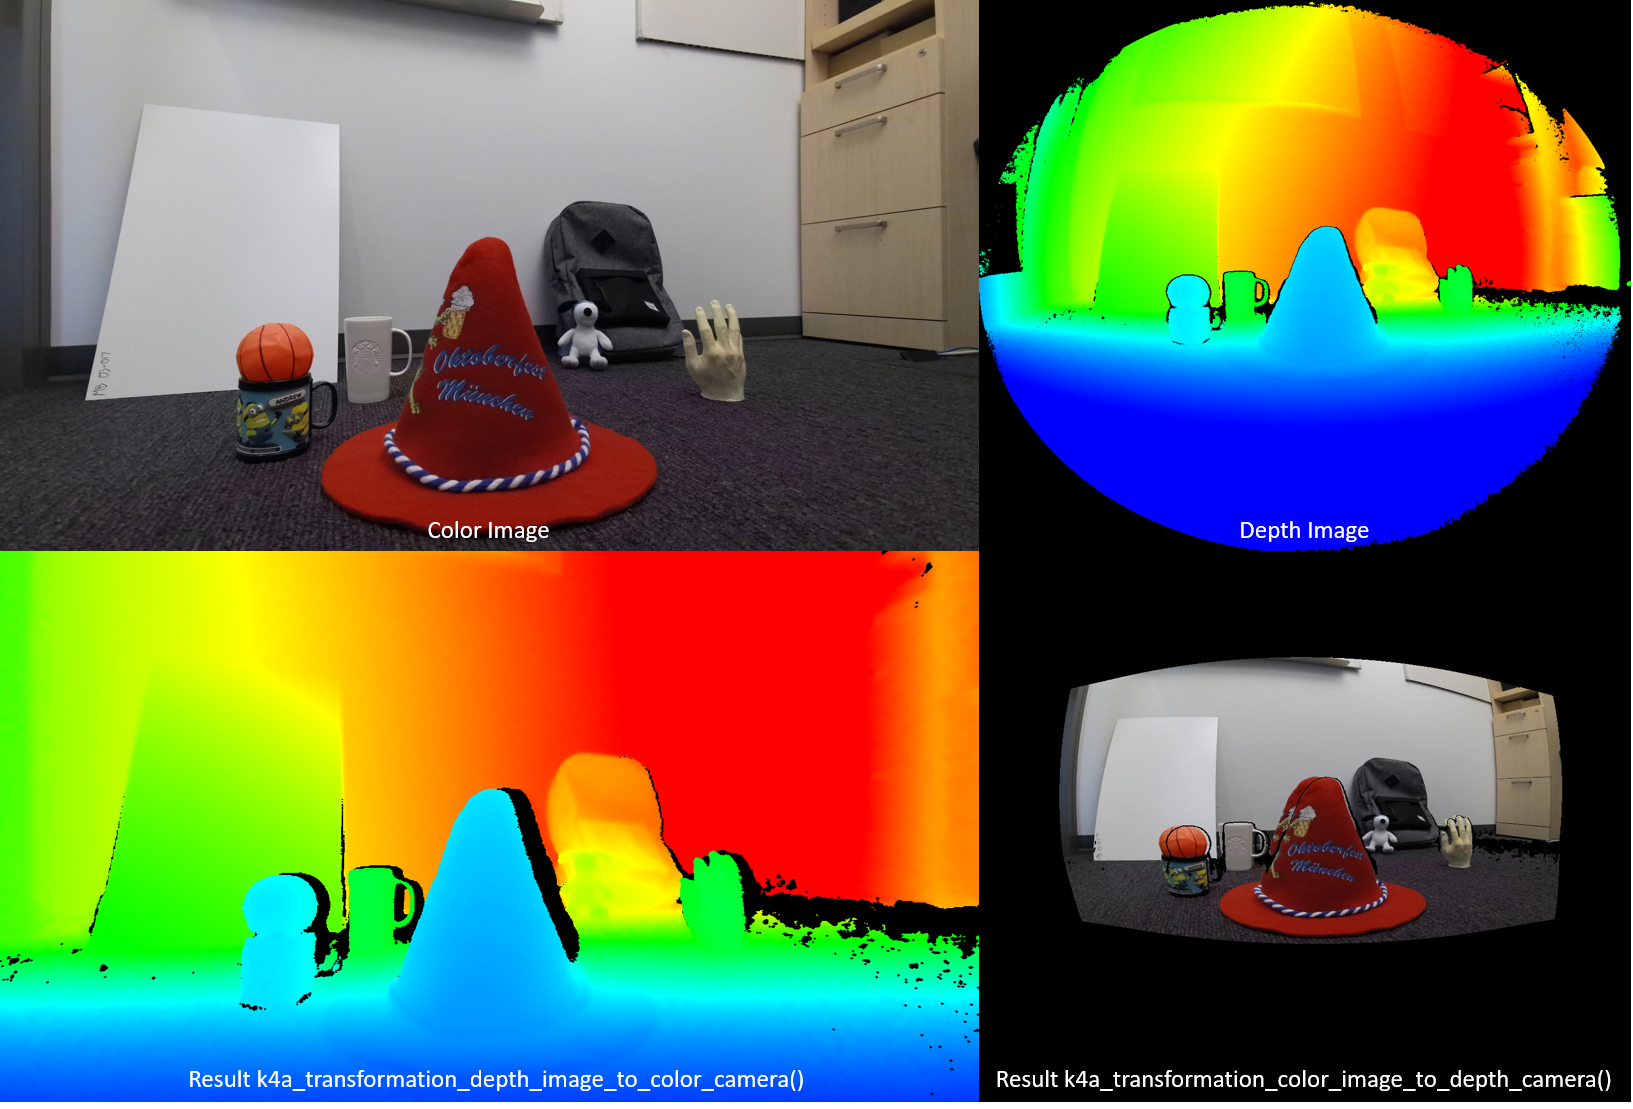
\includegraphics[width = 1.0\linewidth]{./implementation/figures/different spaces.png}
\end{figureBox}


The camera when polled with K4A returns a "Capture" which is a struct containing a colour image, depth image and an IR image. We don't use the IR image in our project so we ignore it. It is worth noting that the depth image is in a different space to the colour image as can be seen in Fig~\ref{fig:diff-spaces}. The depth image is in the "depth space" and the colour image is in the "colour space". To use the two images in conjunction we have to convert them into the same space. \\

Using a "calibration" that is generated at the start of the program k4a lets you convert between the 4 difference "spaces", "Depth 2D", "Depth 3D", "Colour 2D", "Colour 3D". There are interesting performance implications of using different spaces for different tasks. For example going from "Depth 2D" to "Depth 3D" is significantly faster than going from "Colour 2D" to "Colour 3D". \\

Another interesting side effect of converting between spaces if because the IR and colour cameras are physically offset and diffract differently you get "depth shadows" \tocite as can be seen in the Bottom Left image in Fig~\ref{fig:diff-spaces}. Which can make it difficult when trying to track thin objects like fingers as you have a high probability of getting an invalid depth.

\subsubsection{OpenCV}

We use OpenCV to handle the images we get from the Azure Kinect SDK. OpenCV is a library that provides a comprehensive set of functions for image processing and computer vision. We use OpenCV to convert the images we get from the Azure Kinect SDK into a format that can be more easily used by Dlib and MediaPipe. We make use of OpenCV's GPU accelerated functions like to down scaling. To increase the performance of our tracking system. We also use OpenCV for debugging to render the images to the screen.

\subsubsection{Dlib}

We use Dlib to track the user's face. Dlib is a modern C++ toolkit containing machine learning algorithms and tools for creating complex software in C++ to solve real-world problems. We use Dlib's face tracking model \tocite to track the user's face. Dlib's face tracking model is a deep learning model that can track the user's face in real-time. We use Dlib's GPU accelerated functions to increase the performance of our tracking system. We initially used Dlib's CPU face tracking functionality but found that it was bottlenecking our system. We then switched to Dlib's GPU functions and found that it significantly increased the performance of our tracking system. \textcolor{red}{Fill out more}

\subsubsection{MediaPipe}

We use MediaPipe to track the user's hands. MediaPipe is a cross-platform framework for building multi-modal applied machine learning pipelines. We use MediaPipe's hand tracking model \tocite on colour images to track the user's hands. MediaPipe's hand tracking model is a deep learning model that can track the user's hands in real-time. \textcolor{red}{Fill out more}

%%%%%%%%%%%%%%%%%%%%%%%%%%%%%%%%%%%%%%%%%%%%%%%%%%%%%%%%%%%%%%%%%%%%%%%%%%%%%%%%%%%%%%%%%%%%

\subsection{Overall Tracking System Design}

\begin{enumerate}[itemsep=-0.25em]
	\item Diagram of how the system works.
	\item Picture diagram of capture to tracking frame.
	\item Mention how we track the hands and face seperately so two capture frames.  
\end{enumerate}

The purpose of the tracking system in brief strokes is to convert the Captures provided by the Kinect Camera into 3D point representing useful information from the render like the position of the users eye and fingers. The current system just returns the position of the left eye and index and thumb tip on the closest hand to the camera. The system runs as the same speed of as camera (30fps) and feels smooth. \\

There were a number of different approaches we could have taken but in the end we decided to use a system that tracked the position of the users face and hands separately in 2D which we then converted into 3D. The main other approach we could have taken was to track the face and hands in 3D directly. In the end the main reason we decided against this approach was because although the rendering system was a key part of this project it was not the main focus. The main focus was the user study and the tracking system was just a means to an end. The ecosystem for tracking in 2D is much more mature (thanks in part to mobile phones) than in 3D and we were able to leverage a lot of existing work (Such as the previously described libraries Dlib, MediaPipe, and OpenCV). Another reason was that we were concerned about the performance of tracking in 3D. We were worried that tracking in 3D would be too slow to be able to track the users face and hands in real-time, however is suspect this probably would have been fine. There are a number of downsides that arise from tracking in 2D. For example, as we will talk about a bit more in the evaluation section, it is difficult to find the accurate positions of objects in 3D space that are occluded for example fingers behind other fingers. Because fingers are fairly small objects we also have to sample a vague area where we think it is and pick the closet point as if you only sample the predicted point you can miss the finger.\\

\textcolor{red}{Mention what happens when tracking fails (i.e only replace replace images in the frame if successful)}

\begin{figureBox}[label={fig:tracker-overview}, width=1.0\linewidth]{Tracker overview}
    \includegraphics[width = 1.0\linewidth]{./implementation/figures/tracker.pdf}
\end{figureBox}

As can be seen in Fig~\ref{fig:tracker-overview} the basic flow of the tracking system is as follows.
\begin{enumerate}[itemsep=-0.25em]
	\item Retrieve the Capture from the Kinect Camera.
	\item Run hand and head tracking on the colour image.
	\item Extract the key 2D points from the hands (thumb and index tip) and face (left eye).
	\item Use the depth image to convert the 2D points into 3D points and put these in a "tracking frame" to be sent to the rendered.
\end{enumerate}

While it might seem strange at first as can be seen in the Tracking Frame in Fig~\ref{fig:tracker-overview} we actually keep a separate instance for the left eye and the thumb and index tips. This is because there is no guarantee that the tracker will be able to detect both the face and hands at the same time. For example if the user is holding their hand in front of their face the tracker will only be able to detect the hand. If this happens our system will just reuse the last known position which is a good approximation of faces position. 

\subsection{Tracking Models}
\subsubsection{Dlib}
% tocite one: \texttt{https://arxiv.org/abs/1502.00046} 
% tocite two: \texttt{https://blog.dlib.net/2016/10/easily-create-high-quality-object.html}

% tocite three: \texttt{https://ieeexplore.ieee.org/document/6909637}
% tocite four: \texttt{https://ibug.doc.ic.ac.uk/resources/facial-point-annotations/}
We use Dlib to track the eye using a two stage process. In the first stage we use a Max-Margin Object Detection model \tocite \tocite  using a convolutional neural network (CNN) \tocite. Instead of training our own model we used a pertrained model provided by dlib \tocite called \texttt{mmod\_human\_face\_detector}. The initial face detection was a bottlekneck for us, we chose to run our CNN on a GPU using CUDA accelerated functions. \\
 
Once we have detected our face we run the second stage of our facial landmark detection model. We chose to use a 5 landmark pose estimator called \texttt{ shape\_predictor\_5\_face\_landmark} using dlibs implimentation of a method preposed in "One millisecond Face Alignment with an Ensemble of Regression Trees" \tocite{https://ieeexplore.ieee.org/document/6909637} trained on the iBUG 300-W face landmark dataset \tocite. This pose estimator ran fast enough on a CPU that we didn't bother GPU accelerating it. \\

An example of the result of running the dlib two models can be seen in Fig~\ref{fig:head-tracker} \\
\begin{invisBox}  
	\pictureBox[label={fig:Face-tracker}]{Dlib Face Tracker}{
	  \adjustbox{height=5.75cm, keepaspectratio}{
		\includegraphics{./implementation/figures/Face-tracker.png}
	  }
	}
	\hfill
	\pictureBox[label={ig:hand-tracker}]{MediaPipe Hand Tracker}{
	\adjustbox{height=5.75cm, keepaspectratio}{
	  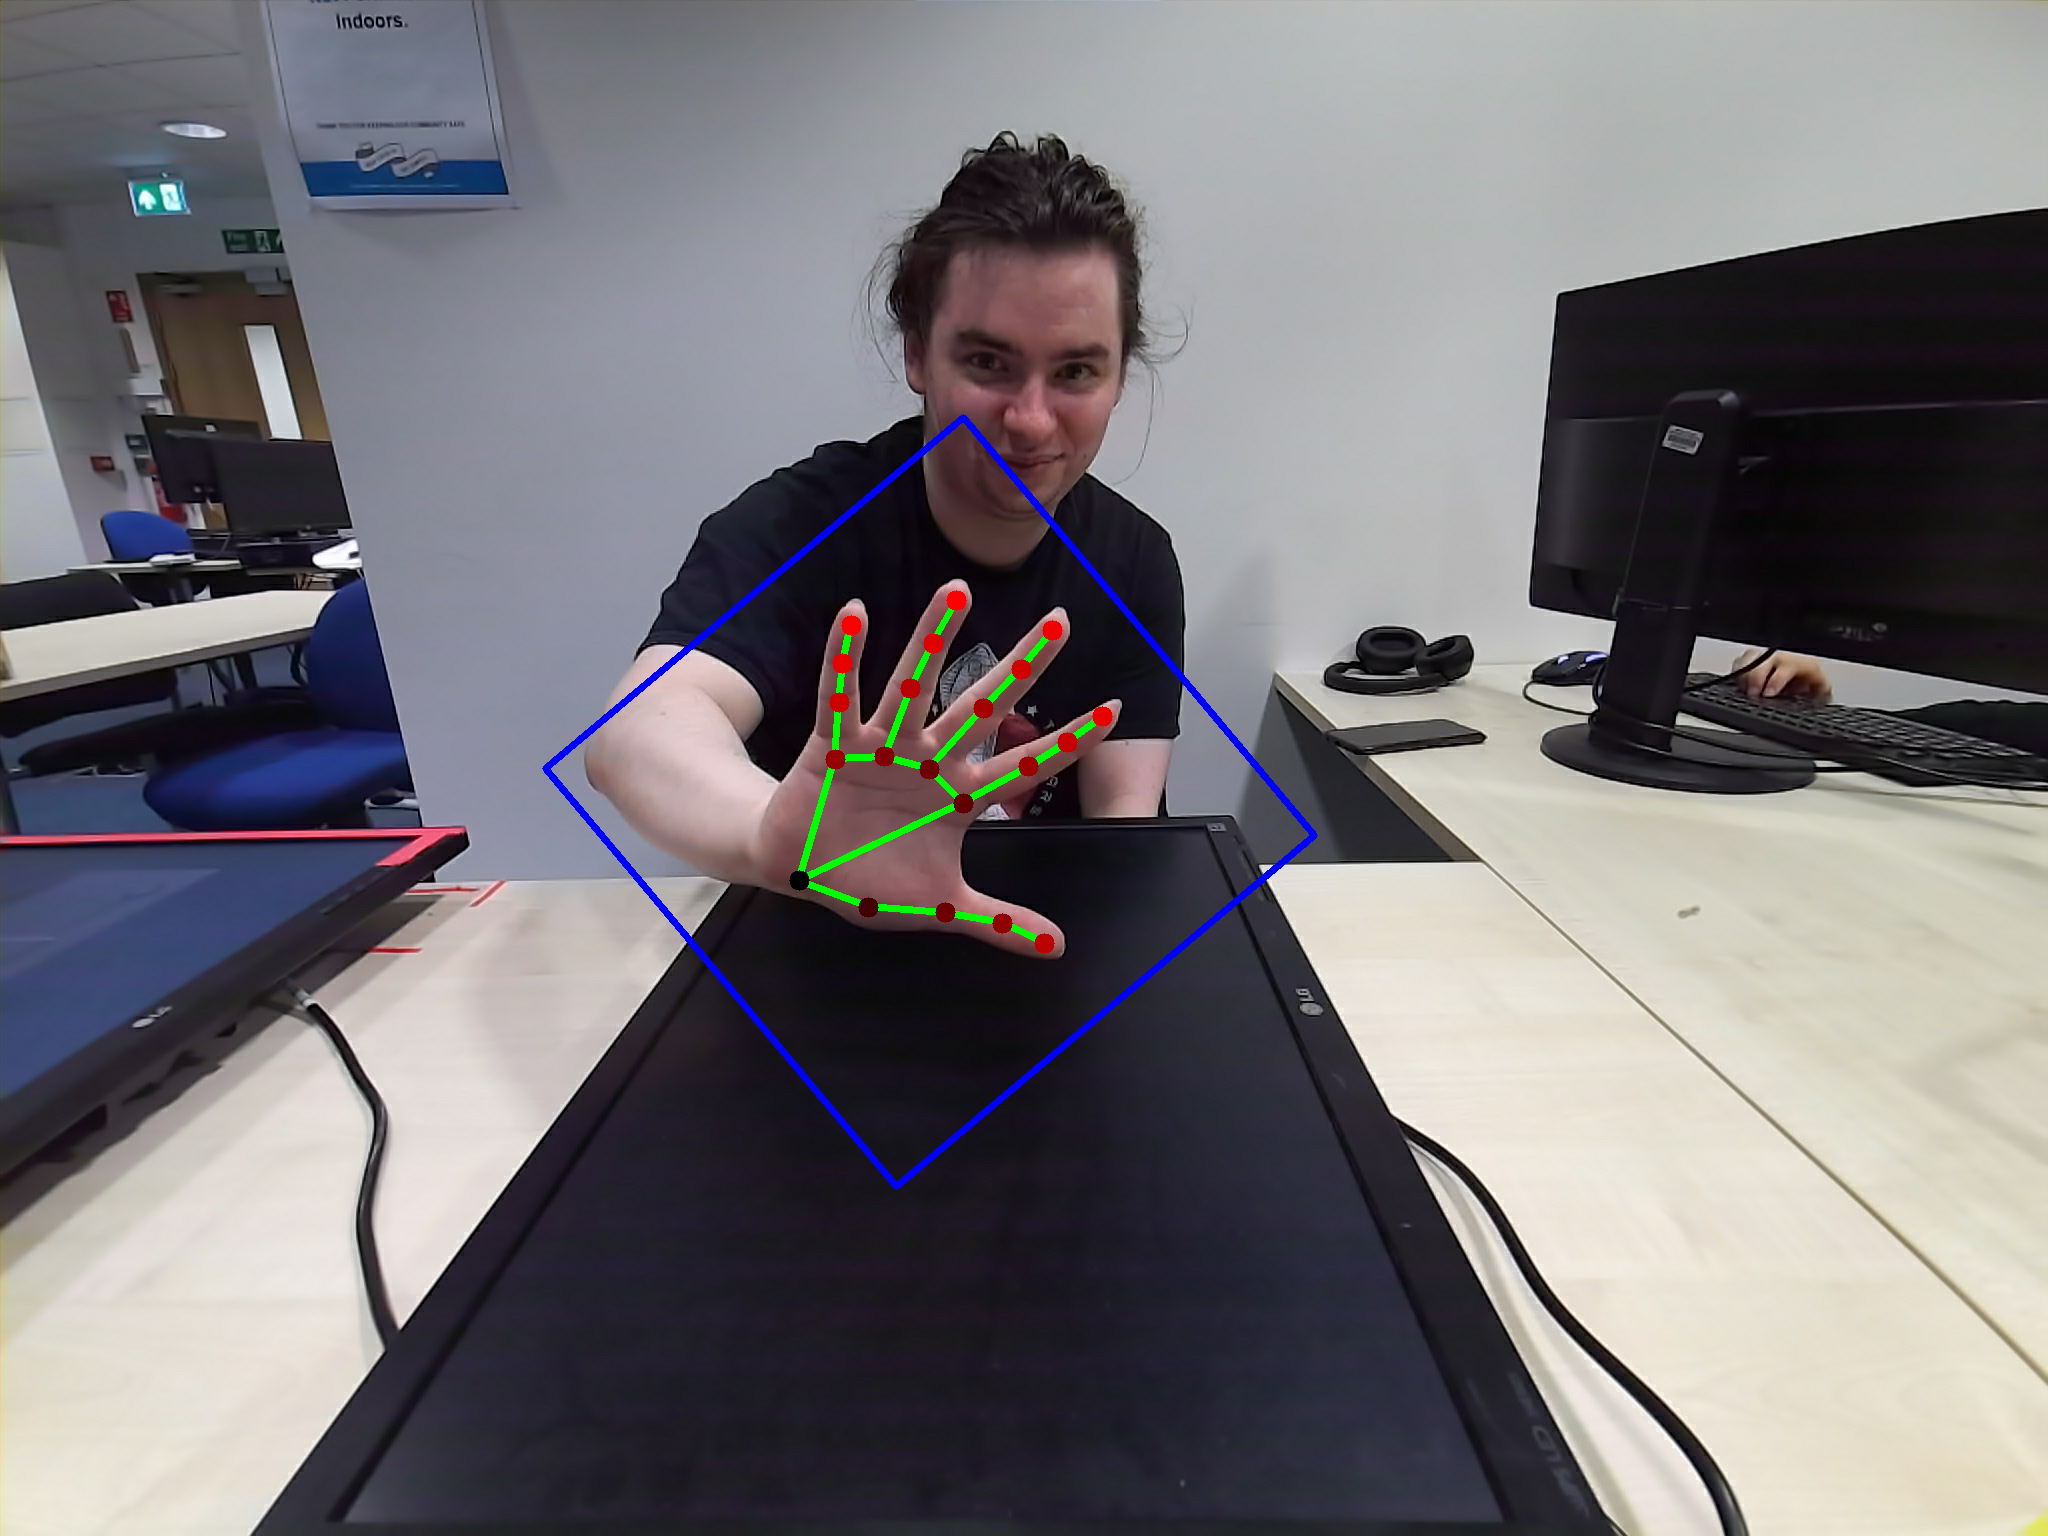
\includegraphics{./implementation/figures/hand-tracker.png}
	  }
	}
\end{invisBox}

% tocite one: \texttt{https://arxiv.org/abs/2006.10214}
We use MediaPipe to track the position of two fingers on the users hand, also using a two step process. MediaPipe uses a two stage model to track the hands \tocite. The first stage is a palm detection model that detects the position of the hand in the image. The second stage is a hand landmark model that detects the position of 21 points on the hand. MediaPipe provides a nice interface to for pushing our images in the form of a stream and abstracts away most detection logic for you unlike dlib. \\

We chose to track the position of the index and the middle finger as we found that this was more stable than tracking the thumb and index finger. Because we depth sample from the surface of the hand we chose to offset the positions by constant amount of make it feel like the point was inside the hand. An example of the result of running the MediaPipe two models can be seen in Fig~\ref{fig:hand-tracker} \\

\subsubsection*{Downscaling}
To make sure our tracking system runs at a high enough framerate we downscale the images we get from the camera. We found that we could downscale the images by a factor of 2 and still get accurate tracking results. This significantly increased the performance of our tracking system. 

%%%%%%%%%%%%%%%%%%%%%%%%%%%%%%%%%%%%%%%%%%%%%%%%%%%%%%%%%%%%%%%%%%%%%%%%%%%%%%%%%%%%%%%%%%%%

\subsection{Multithreading}

\begin{enumerate}[itemsep=-0.25em]
	\item Seperate thread for tracking capturing and rendering
	\item Increased framerate but did not change latency.
	\item More wasteful in terms of resources but there is there are more than enough resources.
	\item Talk about polling architecture and how we cache frames so we don't do redundant work.
\end{enumerate}

\begin{figureBox}[label={fig:mult-threaded-des}, width=0.8\linewidth]{Multi-threaded design}
    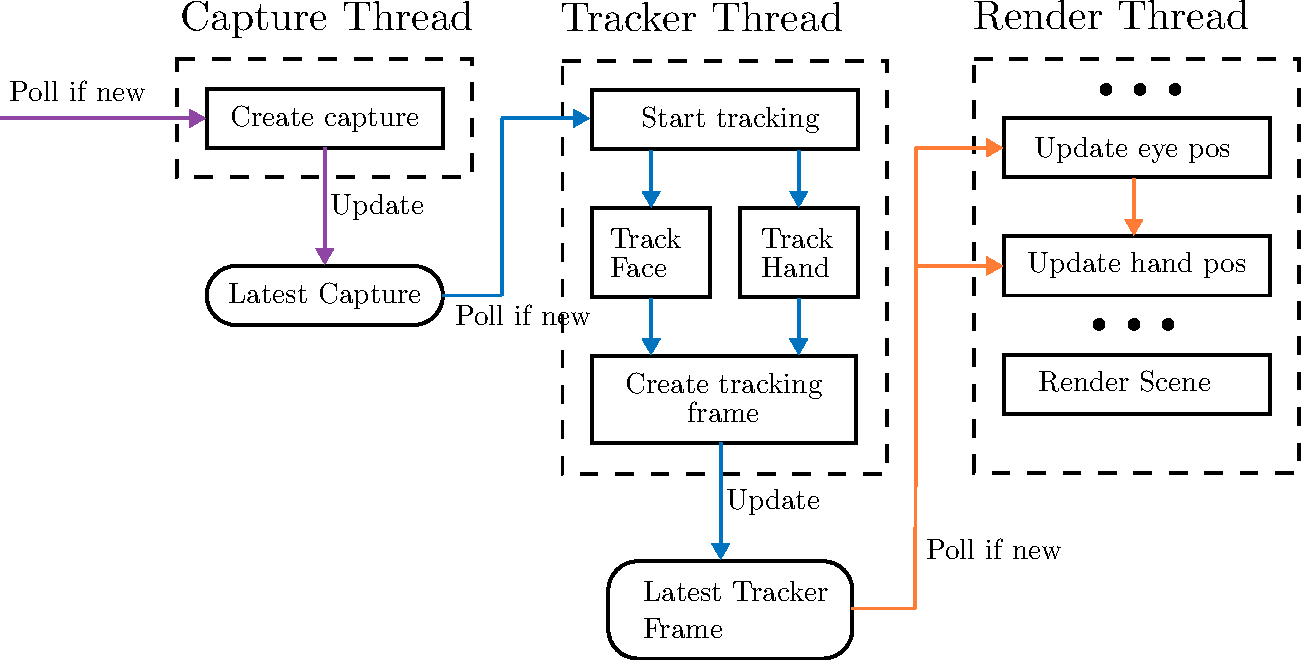
\includegraphics[width = 1.0\linewidth]{./implementation/figures/multi-thread-design.pdf}
\end{figureBox}

One of the more challenging aspects of this project was to make our tracking system run fast enough that it felt smooth. To achieve this we had to make use of multi-threaded design as can be seen in Fig~\ref{fig:mult-threaded-des}. We used a separate thread for tracking, capturing, and rendering. This is a slightly wasteful use of resources as we effectively waste a thread waiting for captures however as the whole simulation is surprisingly light on resources this was not a problem it was worth it for the framerate gain it provided. \\

The purpose of this design choice is to make sure there is always a threading running the tracking models as these are by far the computationally most expensive part of the system. Using a multithreaded design does not reduce the latency (which we talk about more in evaluation) of the system but rather increases the throughput which in our case is the framerate of the application. As we are using a camera that runs at 30fps we need to be able to process an image every $\frac{100\text{ms}}{30\text{ms}} = 33 \text{ms} $. As can be seen in Fig~\ref{fig:single-vs-multi} by switching to a multi-threaded design we can increase the framerate of our whole tracking system to be the same as time required to run our tracking modules on our already retrieved captures. This also gives us the advantage of being able to run the simulation at an independent framerate to the tracker. \\

\textcolor{red}{TO DO ADD KEY, also show how long each individual part takes. Also show that rendering happens multiple times a second}
\begin{figureBox}[label={fig:single-vs-multi}, width=0.8\linewidth]{Single vs Multi threaded design}
    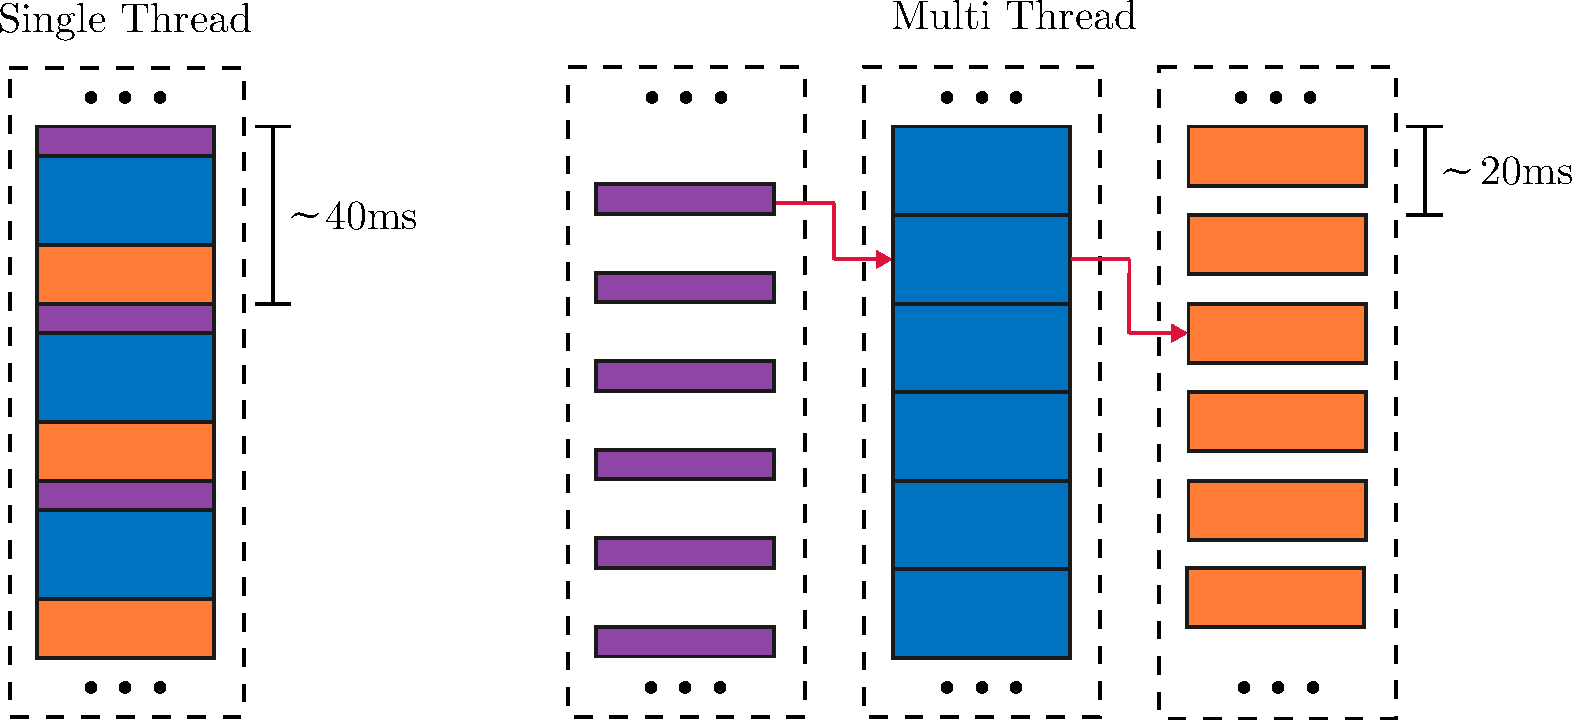
\includegraphics[width = 0.8\linewidth]{./implementation/figures/single-vs-multi.pdf}
\end{figureBox}

%%%%%%%%%%%%%%%%%%%%%%%%%%%%%%%%%%%%%%%%%%%%%%%%%%%%%%%%%%%%%%%%%%%%%%%%%%%%%%%%%%%%%%%%%%%%

\subsection{GPU Acceleration}

Another method we use to increase the performance of our tracking system is to use GPU acceleration. Both Dlib and MediaPipe support GPU acceleration. We only used GPU acceleration in Dlib as we found that it significantly increased the performance of our tracking system. \textcolor{red}{get actual stats for dlib gpu stats}. We did not use GPU acceleration in MediaPipe as the CPU speed was already sufficient and the purported speedup of 12.27ms with GPU acceleration vs 17.12ms \textcolor{red}{to cite https://ai.google.dev/edge/mediapipe/solutions/vision/hand\_landmarker} with cpu only didn't seem worth the effort of enabling CUDA in mediapipe after it already provided difficult to use (See build systems for more information) . We did not test the performance of MediaPipe with GPU acceleration as we did not have the time.  \\

As you can see in Fig~\ref{fig:system-des} we only used GPU acceleration for 3 parts of our tracking system. We downscale our colour images using OpenCV's GPU accelerated pyramid down function as this is a highly parallel task and benefits from the acceleration. We also run the dlib cnn for detecting the face on the GPU. Lastly we run our rendering system on the GPU.
\begin{figureBox}[label={fig:system-des}, width=1.0\linewidth]{Overall Tracking System Design}
    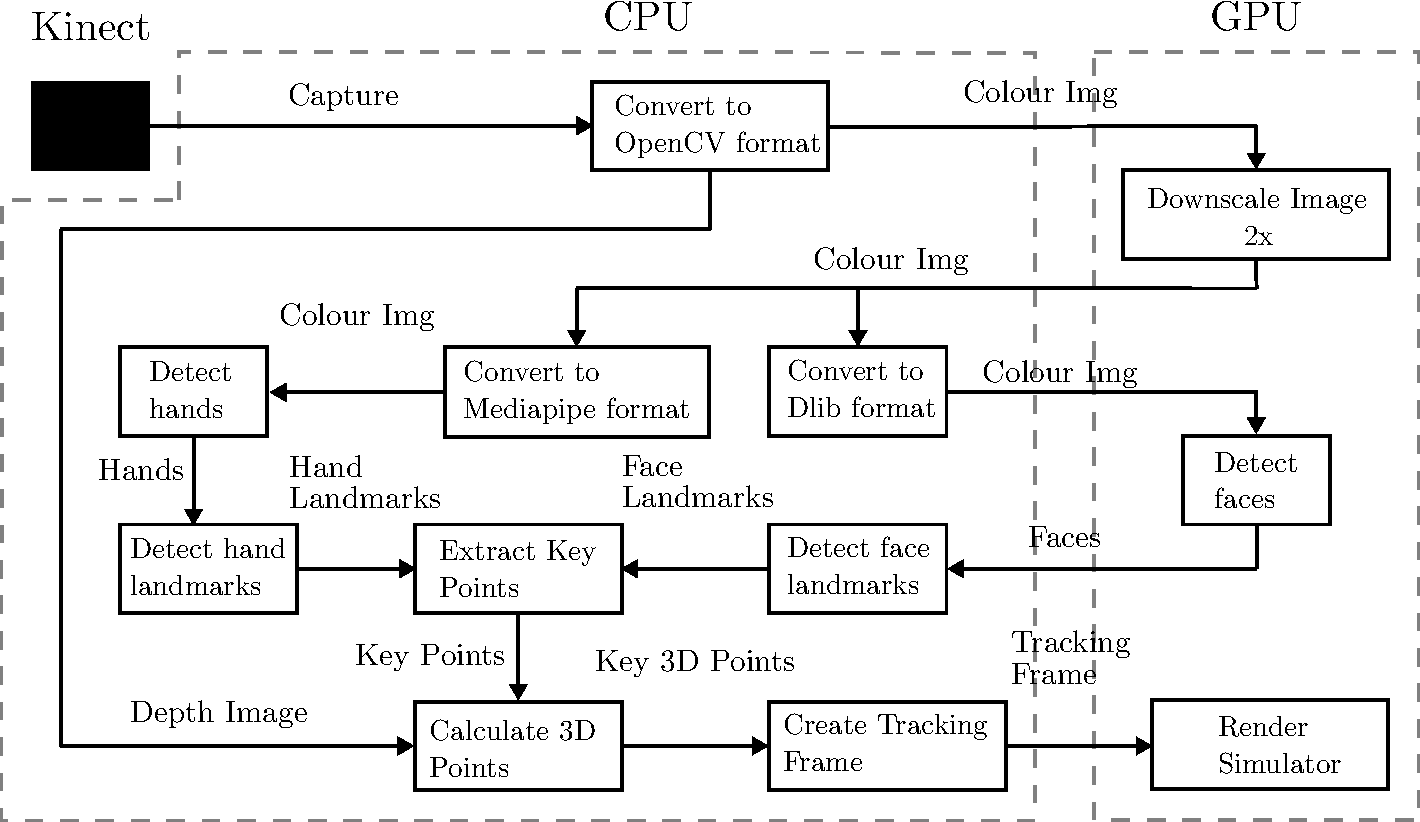
\includegraphics[width = 1.0\linewidth]{./implementation/figures/tracking-system.pdf}
\end{figureBox}

\begin{enumerate}[itemsep=-0.25em]
	\item Dlib and MediaPipe both support GPU acceleration. Only did it in DLIB. Get benchmarks from Mediapipe and DLIB
	\item downscaling to increase performance has the downside of reducing precision/resolution but it was negligible.
\end{enumerate}

%%%%%%%%%%%%%%%%%%%%%%%%%%%%%%%%%%%%%%%%%%%%%%%%%%%%%%%%%%%%%%%%%%%%%%%%%%%%%%%%%%%%%%%%%%%%

\subsection{Camera Positioning}

To set up the tracking system to be calibrated correctly such that the user can see the correct perspective with need to know the relative position of the camera to the screen, the orientation of the camera and the dimensions of the screen. We use a calibration system to set up the camera. The calibration system works as follows:

\begin{enumerate}[itemsep=-0.25em]
	\item Camera is measured in 3D space and orientation is recorded. Screen is measured in 3D space. 
	\item Relative positions are given to the system 
	\item Predicted position of the screen in rendered in 3D.
	\item Iteratively adjust the position of the screen until they line up. 
\end{enumerate}

An example of a correct and incorrect calibration can be seen in Fig~\ref{fig:calibration}

\begin{figureBox}[label={fig:calibration}, width=0.8\linewidth]{Display Calibration}
    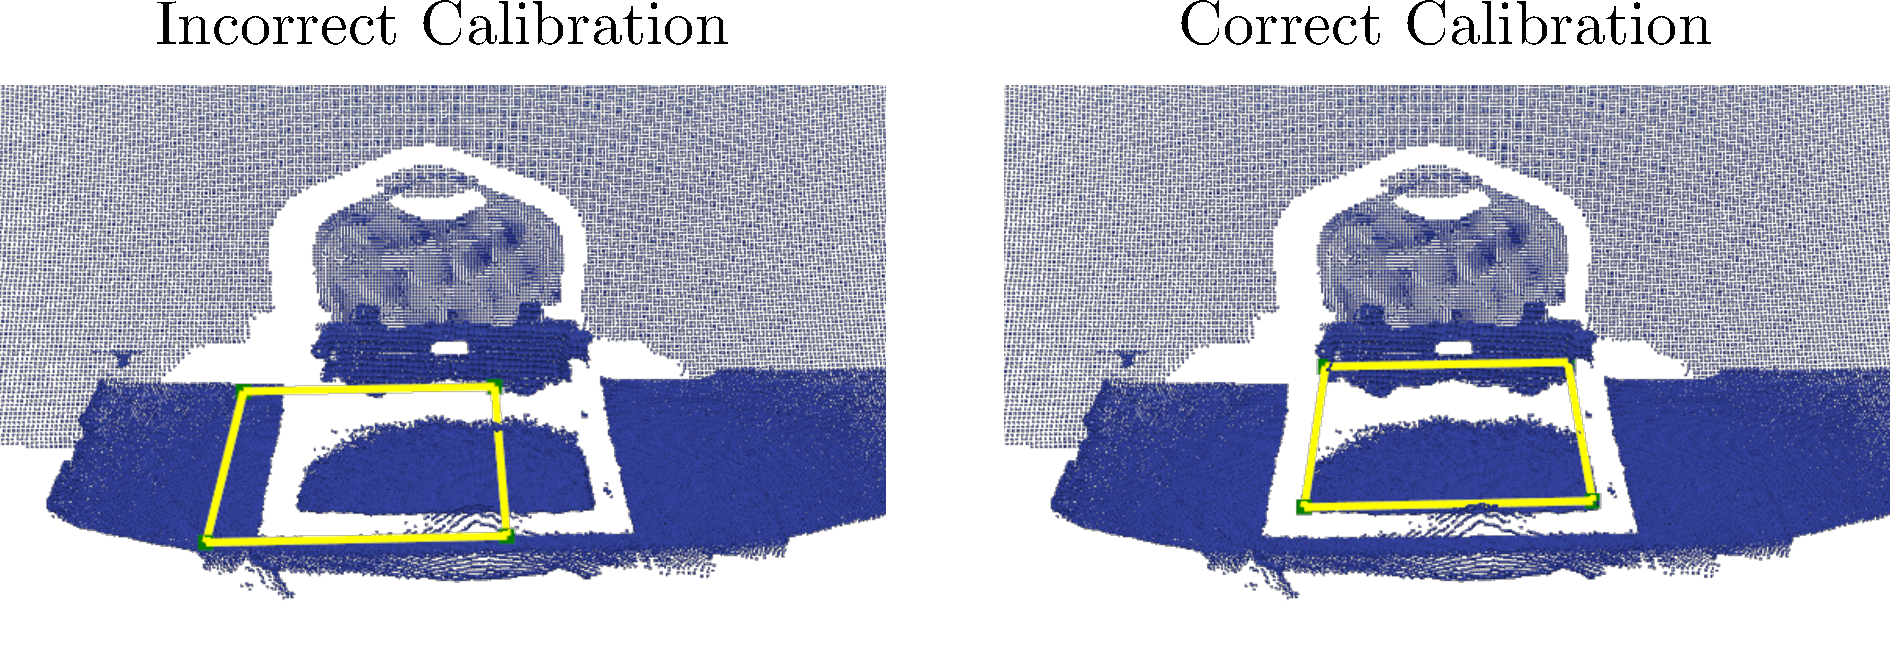
\includegraphics[width = 1.0\linewidth]{./implementation/figures/calibration.pdf}
\end{figureBox}